\section{Tools}\label{tools}


%%%%%%%%%%%%%%%%%%%%%%%%%%%%%%%%%%%%%%%%%%%
\subsection{The Generator}\label{generator}
%%%%%%%%%%%%%%%%%%%%%%%%%%%%%%%%%%%%%%%%%%%
The Generator tool is a graphical user interface developed in Java, allowing the user to store data from OWL files into a MySQL database. This tool also permits the user to query the database using the C++ function calls. The tool Generator is composed of the following functionalities:
\begin{enumerate}
 \item Convert OWL documents into SQL syntaxes (OWL to SQL).
 \item Translate SQL syntaxes to OWL language in order to modify an OWL document (SQL to OWL).
 \item Convert the OWL language into C++ classes (OWL to C++).
\end{enumerate}

To date, only steps 1. and 3. have been implemented and will be covered in this document.

\subsubsection{Prequisites}\label{s:prequisites}
The description of the Generator tool is given for a Ubuntu Linux system. To run and use the Generator tool, different applications must be installed on the system.

\paragraph{Java Runtime Environment}
The Generator tool comes as a jar file. As such, the Java Runtime Environment should be installed on your system. This application can be found at \url{www.oracle.com}.

\paragraph{MySQL Server and Client}
The MySQL server and client should be installed and running on your system.
\begin{itemize}
 \item \textit{sudo apt-get update} (Update the package management tools)
 \item \textit{sudo apt-get dist-upgrade} (Install the latest software)
 \item \textit{sudo apt-get install mysql-server mysql-client} (Install the MySQL server and client packages). You will be asked to enter a password.
\end{itemize}

When done, you have a MySQL database ready to run. The following command will allow you to run MySQL.

\begin{itemize}
 \item \textit{mysql -u root -p}
 \item Enter the same password you used when you installed MySQL.
\end{itemize}

Finally, we need the plugin \texttt{libmysqlcppconn-dev} which allows C++ to connect to MySQL databases. It can be installed as follows:
\begin{itemize}
 \item \textit{sudo apt-get install libmysqlcppconn-dev}
\end{itemize}

\subsubsection{How to Run the Generator Tool}\label{s:run}
The Generator tool can be launched using either one of these two following methods:
\begin{enumerate}
 \item \textit{java -jar Generator.jar}
 \item Right-click on Generator.jar and select the option ``Open With OpenJDK Java 6 Runtime". Note that this message will be different for future releases of the Java Runtime Environment.
\end{enumerate}


\subsubsection{Functionalities}\label{s:generator}
As mentioned in the Introduction, we are covering only steps 1. and 3. in the rest of this document, i.e., \textit{OWL to SQL} and \textit{OWL to C++}, respectively.

\paragraph{OWL to SQL}
\begin{figure}[h!t!]
\centering
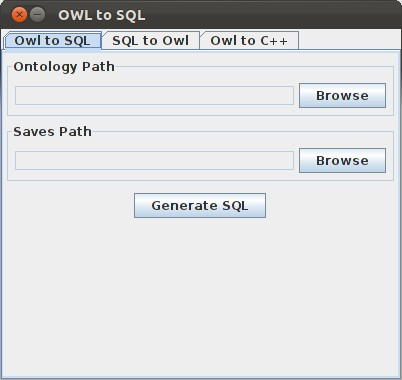
\includegraphics[width=9cm]{Figure/OWLtoSQL001.jpeg}
\caption{Owl to SQL tab.}
\label{fig:owl2sql}
\end{figure}
To convert OWL classes and instances to SQL, the \texttt{Owl to SQL} tab should be selected (see Figure~\ref{fig:owl2sql}). The different fields are:

\subparagraph{Generate SQL Files}
\begin{itemize}
 \item Ontology Path: This field requires the file \texttt{kittingInstances.owl}. Before doing so, you need to modify one line in this file. Open it with a text editor and find the line \texttt{Import(<file:kittingClasses.owl>)}. Modify
this line by giving the absolute path to the file \texttt{kittingClasses.owl}. You should should have something that looks like \texttt{Import(<file:/home/username/NIST/ipmas/Generator/kittingClasses.owl>)}. When this is done, save the file, and browse to  \texttt{kittingInstances.owl} using the ``Browse" button.
 \item Browse to the directory where you want to save the SQL files.
\end{itemize}

Once the two previous steps are done, click on ``Generate SQL''. You should receive a message confirming the generation of the SQL files: \texttt{kittingInstances.owlCreateTable.sql} and \texttt{kittingInstances.owlInsertInto.sql}. The former is used to create tables, the latter is used to populate these tables;

\subparagraph{SQL Tables and Insertions}
The next step is to create a database and to populate it.

\begin{itemize}
\item Connect to mysql using \textit{mysql -u root -p}, then enter your password. You should be in the mysql shell if this succeeded (\textit{mysql>}).
\item Delete a previous database (if you already used this tool and you want to replace the existing database with this new one) :
\texttt{mysql>} \textit{DROP DATABASE OWL;} (\textit{OWL} is the name of the old database).
\item Create a database:
\begin{itemize}
\item \texttt{mysql>} \textit{CREATE DATABASE OWL;}. Here, \textit{OWL} is the name of the database (you can use a name of your choice).
\item Before performing the following commands, we need to tell MySQL which database we are planning to work with (\textit{OWL} in our case). This is done using:
\begin{itemize}
\item[] \texttt{mysql>} \textit{USE OWL}
\end{itemize}
\end{itemize}
\item Populate the database with tables using \texttt{kittingInstances.owlCreateTable.sql}.
\begin{itemize}
 \item \texttt{mysql>} \textit{source <path>/kittingInstances.owlCreateTable.sql;}
\end{itemize}

\item Populate the tables with data using \texttt{kittingInstances.owlInsertInto.sql}:
\begin{itemize}
 \item \texttt{mysql>} \textit{source <path>/kittingInstances.owlInsertInto.sql;}
\end{itemize}
\end{itemize}

\textit{<path>} designs the absolute path to the appropriate file.

\paragraph{OWL to C++}
\begin{figure}[h!t!]
\centering
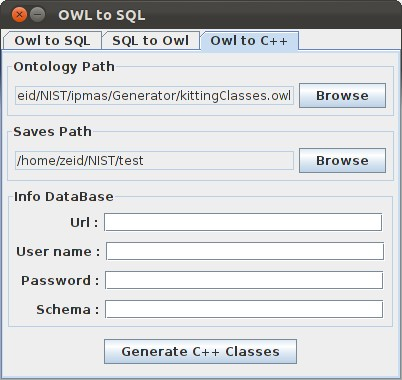
\includegraphics[width=9cm]{Figure/OWL2C++.jpeg}
\caption{Owl to C++ tab.}
\label{fig:owl2C++}
\end{figure}
The ``Owl to C++" tab (see Figure~\ref{fig:owl2C++}) is used to generate C++ classes and scripts allowing the connection between C++ and MySQL. The different fields are explained below:
\begin{itemize}
\item \textbf{Ontology Path}: This is the path to the ontology (\texttt{kittingClasses.owl} in our example).
\item \textbf{Saves Path}: Directory where the C++ files and scripts will be generated.
\item \textbf{Url}: This is the url of the database. It's usually the IP address of the machine hosting the database (127.0.0.1 if it is local).
\item \textbf{User name}: User name used to connect to the MySQL database.
\item \textbf{Password}: Password associated to the user name to connect to the MySQL database.
\item \textbf{Schema}: This is the name of the database (\textit{OWL} in our example).
\end{itemize}

When all the fields are completed, click the ``Generate C++ Classes" button to generate C++ and script files.

%%%%%%%%%%%%%%%%%%%%%%%%%%%%%%%%%%%%%%%%%%%
\subsection{XML to OWL}\label{xml2owl}
%%%%%%%%%%%%%%%%%%%%%%%%%%%%%%%%%%%%%%%%%%%
This section describes tools that are used to generate OWL files from XML files.
\subsubsection{owlPrinter}
owlPrinter reads an XML kitting data file corresponding to an XML schema for kitting (\file{kitting.xsd}) and writes an OWL instance file corresponding to the OWL class file \file{kittingClasses.owl}. The \file{kitting.xsd} file contains the same conceptual model as the \file{kittingClasses.owl} file, but in a different language.

The owlPrinter is useful because there is no OWL tool that will help generate an OWL instance file and check the file adequately against an OWL class file. That is because OWL uses an open world model in which anything not explicitly or implicitly illegal is allowed. Hence many things that are errors to the writer of the instance file are not OWL errors. For example, if the name of an instance is misspelled, OWL will assume that there is a new instance that has not been explicitly declared as such, which is OK in OWL. If a reference to an instance name is misspelled in an XML data file corresponding to the \file{kitting.xsd} schema, that will be caught automatically by the owlPrinter (and other readily available XML tools).  Several other types of error will not be caught by OWL tools but will not be made or will be detected if the OWL printer is used.

Another OWL problem that disappears in XML is that in OWL, there is no distinction between an instance file and a class file. An instance file can modify classes, intentionally, or accidentally. In XML there is no way a data file can modify a model.

To use the owlPrinter, use a text editor such as emacs or an XML tool such as XMLSpy to write an XML data file corresponding to the \file{kitting.xsd} schema and then run it through the owlPrinter with a command of the form:\\

\texttt{bin/owlPrinter [XML file in] [OWL file out]}\\

For example, the command\\

\texttt{bin/owlPrinter data/kittingInstances.xml junk}\\

will print the file junk, which will be identical to the \file{kittingInstances.owl} file in the owl directory (except for a couple comments).


\subsubsection{kittingParser}
The kittingParser may be used to check an XML data file against the
kitting.xsd schema. The schema is hard-coded into the kittingParser.
If there is any error in the XML data file, the kittingParser prints
a message and quits. If there is no error, the input file is echoed by
printing an output file whose name is the same as that of the input file
with "echo" appended. To run the kittingParser, give a command of the
form:\\
\texttt{bin/kittingParser [XML kitting data file in]}\\

For example, the command\\

\texttt{bin/kittingParser data/kittingInstances.xml}

will read \file{kittingInstances.xml} and write \file{kittingInstances.xmlecho}. The
two files will be identical except for comments. If the format of an
input file differs from the format used for printing the output file,
the two files will differ, but only in format.

The owlPrinter makes the same checks as the kittingParser, so there is
no need to use the kittingParser.

All of the source code for the kittingParser was generated automatically
by the GenXMiller generator.

\subsubsection{compactOwl and compareOwl}
There is no need to read this section unless you are interested in how the
\app{owlPrinter} was debugged.

The \app{compactOwl} and \app{compareOwl} utilities are used for checking that two
different OWL instance files have the same statements. They have been
used as follows to debug the \app{owlPrinter} (and the \file{kitting.xsd} file
and the \file{kittingInstances.xml} file and the \file{kittingInstances.owl} file).

\begin{enumerate}
\item Write \file{kitting.xsd} to model the same information as \file{kittingClasses.owl}.

\item Write \file{kittingInstances.xml} to correspond to \file{kitting.xsd} and contain the
same information as \file{kittingInstances.owl}.

\item Build the \app{owlPrinter}.

\item Run \file{kittingInstances.xml} through the \app{owlPrinter} to produce
\file{kittingInstances.owl}.

\item Run \file{kittingInstances.owl} through \app{compactOwl} to produce
one version of \file{kittingInstancesCompact.owl}.

\item Run \file{kittingInstances.owl} through \app{compactOwl} to produce
a second version of \file{kittingInstancesCompact.owl}.

\item Run the two versions of \file{kittingInstancesCompact.owl} through
\app{compareOwl}. If \app{compareOwl} reports that the two files have the same
statements, that means that steps 1, 2, and 3 have been done correctly, so
debugging is finished. If \app{compareOwl} reports a pair of statements that
differ, figure out why, go back to step 1, 2, or 3 (or edit
\file{kittingInstances.owl}), fix the problem, and repeat the subsequent steps.
\end{enumerate}

These utilities assume that the format of the input files is the same
as either the format used by the \app{owlPrinter} or the format followed by
the \file{kittingInstances.owl} file. If the format used by an input file is
different from both of those, the utilities may fail.

The \app{compactOwl} utility compacts an OWL instance file by:
\begin{enumerate}
\item removing all occurrences of one or two blank lines. The blank lines
   must not contain spaces or tabs.
\item removing comments. The comments must have ``//'' as the first two
   characters on the line.
\item combining each OWL statement written on two or more lines so it is
   all on one line. The first non-space character on the second line
   must be a colon (:) or a double quote (").
\item rewriting numbers with decimal points so there are exactly six decimal
   places. Such numbers must have at least one digit on each side of the
   decimal point in the input file.
\item putting the \textbf{DifferentIndividuals} inside \textbf{DifferentIndividuals} statements
   into alphabetical order.
\end{enumerate}
To run \app{compactOwl} use a command of the form:\\

\texttt{bin/compactOwl < [owl file in] > [owl file out]}\\

where \texttt{[owl file in]} and \texttt{[owl file out]} are replaced by file names.

The \app{compareOwl} utility compares two files that are expected to have the
same lines, but in a different order, such as an automatically generated
OWL file and a hand-written OWL file. It reads the two files and saves the
lines of each one in two sets in alphabetical order (set::insert puts
strings in alphabetical order by default). Then it compares the lines of
the two sets in order. If it finds two lines that do not match, it prints
the line from the first file followed by the line from the second file.  If
all lines match, that is reported.

To run \app{compareOwl}, use a command of the form:\\

\texttt{bin/compareOwl [first owl file in] [second owl file in]}

where \texttt{[first owl file in]} and \texttt{[second owl file in]} are replaced by the
names of compacted OWL files.
